\documentclass{beamer}

\usepackage{amssymb,amsmath}
\usepackage{graphicx}
\usepackage{url}
\usepackage{color}
\usepackage{relsize}		% For \smaller
\usepackage{url}			% For \url
\usepackage{epstopdf}	% Included EPS files automatically converted to PDF to include with pdflatex
\usepackage{pagenote}[continuous,page]

%For MindMaps
% \usepackage{tikz}%
% \usetikzlibrary{mindmap,trees,arrows}%

%%% Color Definitions %%%%%%%%%%%%%%%%%%%%%%%%%%%%%%%%%%%%%%%%%%%%%%%%%%%%%%%%%
%\definecolor{bordercol}{RGB}{40,40,40}
%\definecolor{headercol1}{RGB}{186,215,230}
%\definecolor{headercol2}{RGB}{80,80,80}
%\definecolor{headerfontcol}{RGB}{0,0,0}
%\definecolor{boxcolor}{RGB}{186,215,230}

%%% Save space in lists. Use this after the opening of the list %%%%%%%%%%%%%%%%
%\newcommand{\compresslist}{
%	\setlength{\itemsep}{1pt}
%	\setlength{\parskip}{0pt}
%	\setlength{\parsep}{0pt}
%}

%\setbeameroption{show notes on top}

% You should run 'pdflatex' TWICE, because of TOC issues.

% Rename this file.  A common temptation for first-time slide makers
% is to name it something like ``my_talk.tex'' or
% ``john_doe_talk.tex'' or even ``discrete_math_seminar_talk.tex''.
% You really won't like any of these titles the second time you give a
% talk.  Try naming your tex file something more descriptive, like
% ``riemann_hypothesis_short_proof_talk.tex''.  Even better (in case
% you recycle 99% of a talk, but still want to change a little, and
% retain copies of each), how about
% ``riemann_hypothesis_short_proof_MIT-Colloquium.2000-01-01.tex''?

\mode<presentation>
{
  % A tip: pick a theme you like first, and THEN modify the color theme, and then add math content.
  % Warsaw is the theme selected by default in Beamer's installation sample files.

  %%%%%%%%%%%%%%%%%%%%%%%%%%%% THEME
  %\usetheme{Madrid}		% No subsection
  \usetheme{AnnArbor}  % Subsection on top, no color


  %\usetheme{Antibes}
  %\usetheme{Bergen}
  %\usetheme{Berkeley}		% bem bacana - menu esquerdo
  %\usetheme{Berlin}
  %\usetheme{Boadilla}
  %\usetheme{boxes}
  %\usetheme{CambridgeUS}		% bem bacana - menu superior
  %\usetheme{Copenhagen}
  %\usetheme{Darmstadt}
  %\usetheme{default}
  %\usetheme{Dresden}
  %\usetheme{Frankfurt}
  %\usetheme{Goettingen}
  %\usetheme{Hannover}		% bem bacana - menu esquerdo
  %\usetheme{Ilmenau}
  %\usetheme{JuanLesPins}
  %\usetheme{Luebeck}
  %\usetheme{Malmoe}
  %\usetheme{Marburg}		% bem bacana - menu direito
  %\usetheme{Montpellier}
  %\usetheme{PaloAlto}		% bem bacana - menu esquerdo
  %\usetheme{Pittsburgh}
  %\usetheme{Rochester}		%bacana
  %\usetheme{Singapore}
  %\usetheme{Szeged}
  %\usetheme{Warsaw}

  %%%%%%%%%%%%%%%%%%%%%%%%%%%% COLOR THEME
  %\usecolortheme{default}		% branco, azul clarinho
  \usecolortheme{crane}		% Very yellow (ok)

  %\usecolortheme{albatross}		% azul escuro, massa
  %\usecolortheme{beetle}		% cinza, menu azul
  %\usecolortheme{dolphin}		% azul e branco, legal
  %\usecolortheme{dove}			% cinza e branco, feio
  %\usecolortheme{fly}			% todo cinza, horrível
  %\usecolortheme{lily}			% parece o default
  %\usecolortheme{orchid}		% azul e branco, ok
  %\usecolortheme{rose}			% branco e violeta-claro, bonito
  %\usecolortheme{seagull}		% cinza, feio
  %\usecolortheme{seahorse}		% nhé, meio feio
  %\usecolortheme{sidebartab}		% Azul, branco, destaque na tab, interessante
  %\usecolortheme{structure}		% bichado
  %\usecolortheme{whale}		% Azul e branco, bem bonito

  %%%%%%%%%%%%%%%%%%%%%%%%%%%% OUTER THEME
  \useoutertheme{default}
  %\useoutertheme{infolines}
  %\useoutertheme{miniframes}
  %\useoutertheme{shadow}
  %\useoutertheme{sidebar}
  %\useoutertheme{smoothbars}
  %\useoutertheme{smoothtree}
  %\useoutertheme{split}
  %\useoutertheme{tree}

  %%%%%%%%%%%%%%%%%%%%%%%%%%%% INNER THEME
  \useinnertheme{circles}
  %\useinnertheme{default}
  %\useinnertheme{inmargin}
  %\useinnertheme{rectangles}
  %\useinnertheme{rounded}

  %%%%%%%%%%%%%%%%%%%%%%%%%%%%%%%%%%%

  \setbeamercovered{invisible} % or whatever (possibly just delete it)
  % To change behavior of \uncover from graying out to totally
  % invisible, can change \setbeamercovered to invisible instead of
  % transparent. apparently there are also 'dynamic' modes that make
  % the amount of graying depend on how long it'll take until the
  % thing is uncovered.

}


% Get rid of nav bar
\beamertemplatenavigationsymbolsempty

% Use short top
%\usepackage[headheight=12pt,footheight=12pt]{beamerthemeboxes}
%\addheadboxtemplate{\color{black}}{
%\hskip0.5cm
%\color{white}
%\insertshortauthor \ \ \ \
%\insertframenumber \ \ \ \ \ \ \
%\insertsection \ \ \ \ \ \ \ \ \ \ \ \ \ \ \ \ \  \insertsubsection
%\hskip0.5cm}
%\addheadboxtemplate{\color{black}}{
%\color{white}
%\ \ \ \
%\insertsection
%}
%\addheadboxtemplate{\color{black}}{
%\color{white}
%\ \ \ \
%\insertsubsection
%}

% Insert frame number at bottom of the page.
% \usefoottemplate{\hfil\tiny{\color{black!90}\insertframenumber}}

%% makes the ppagenote command for figure references at the end.

\usepackage[english]{babel}
%qq\usepackage[latin1]{inputenc}
\usepackage{CJKutf8}
\usepackage{subfigure}

\usepackage{times}
\usepackage[T1]{fontenc}

\makepagenote
\renewcommand{\notenumintext}[1]{}
\newcommand{\ppagenote}[1]{\pagenote[Page \insertframenumber]{#1}}

\title[Programming Challenges]{GB20602 - Programming Challenges}
\author[Claus Aranha]{Claus Aranha\\{\footnotesize caranha@cs.tsukuba.ac.jp}}
\institute[U. Tsukuba]{University of Tsukuba, Department of Computer Sciences}

\usepackage{tikz}
\usetikzlibrary{arrows,shapes}
% Latex Graph Example:
% https://www.overleaf.com/5297501zrjzfm#/16716638/


\tikzstyle{vertex}=[circle,fill=black!25,minimum size=10pt,inner sep=0pt]
\tikzstyle{blue vertex}=[circle,fill=blue!100,minimum size=10pt,inner sep=0pt]
\tikzstyle{red vertex}=[circle,fill=red!100,minimum size=10pt,inner sep=0pt]
%\tikzstyle{label}=[thin, draw=black, align=center,minimum width=0.5cm, minimum height=0.5cm,fill=white]
\tikzstyle{edge} = [draw,thick,-]
\tikzstyle{red edge} = [draw, line width=5pt,-,red!50]
\tikzstyle{black edge} = [draw, line width=5pt,-,black!20]
\tikzstyle{weight} = [font=\smaller]

\title[GB21802]{GB21802 - Programming Challenges}
\subtitle[]{Week 5 - Graph Problems (Part I)}
\author[Claus Aranha]{Claus Aranha\\{\footnotesize caranha@cs.tsukuba.ac.jp}}
\institute{College of Information Science}
\date{2015-05-27,30\\{\tiny Last updated \today}}

\begin{document}

\section{Introduction}
\subsection{Title}
\begin{frame}
\maketitle
\end{frame}

\subsection{Notes and Warnings}

\begin{frame}
  \frametitle{Last Week Results}
  \begin{columns}[T]
    \column{0.5\textwidth}
    \begin{block}{Week 3 - DP I}
      \begin{itemize}
      \item Jill Rides Again - 15/32
      \item Maximum Sum - 4/32
      \item SDI (rockets) - 8/32
      \item Is Bigger Smarter - 12/32
      \item Ferry Loading - 2/32
      \item Unidirectional TSP - 5/32
      \item Flight Planner 3/32
      \item e-Coins 3/32
      \end{itemize}
    \end{block}
    \column{0.5\textwidth}
    \begin{block}{Week 4 - DP II (At Deadline)} 
      \begin{itemize}
      \item Collecting Beepers - 9/32
      \item Shopping Trip - 1/32
      \item Bar Codes - 7/32
      \item Cutting Sticks - 4/32
      \item String Popping - 2/32
      \item Divisibility - 3/32
      \item Marks Distribution - 8/32
      \item Squares - 3/32
      \end{itemize}
    \end{block}
  \end{columns}
\end{frame}

\begin{frame}
  \frametitle{Special Notes}
\end{frame}

\begin{frame}
  \frametitle{Week 5 and 6 -- Outline}
  {\smaller
  \begin{block}{This Week - Graph I}
    \begin{itemize}
    \item Graph Basics review: Concepts and Data Structure;
    \item Depth First Search and Breadth First Search;
    \item Problems you solve with DFS and BFS;
    \item Minimum Spanning Tree: Kruskal and Prim Algorithms \alert{(Monday)};
     \end{itemize}
  \end{block}
  \begin{block}{Next Week - Graph II}
    \begin{itemize}
    \item Single Sourse Shortest Path (Djikstra);
    \item All Pairs Shortest Path (Floyd Warshall);   
    \item Network Flow and related Problems;
    \item Bipartite Graph Matching and related Problems;
    \end{itemize}
  \end{block}}
  Many variations in graph problems!
\end{frame}

%%% Simple Concepts in Graph Theory
\section{Graph Basics}
\subsection{A Quick Review}

\begin{frame}
  \frametitle{Quick Review of Graph Terms (1)}
  {\smaller
    \begin{block}{}
      You probably know all of these. If not, ask questions!
    \end{block}

    \begin{columns}[T]
      \column{0.6\textwidth}
      \begin{itemize}
      \item A Graph $G$ is made of a set of \structure{vertices} $V$
        and \structure{edges} $E$.
      \item Edges can be \structure{directed}\\ (has source and destination vertices);
      \item Edges can be \structure{weighted} or not\\ (all weigths = 1);
      \item Sets of nodes can be \structure{connected}\\ or \structure{disconnected}
      \item Directed Graphs can be \structure{Strongly Connected}
      \item Edges can be \structure{self-edges}, and/or \structure{multiple edges}
      \end{itemize}
      \column{0.4\textwidth}

      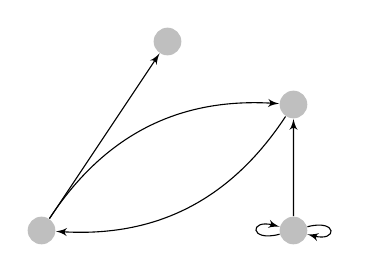
\begin{tikzpicture}[scale=.8,auto,swap]
        \tikzset{edge/.style = {->,>=latex'}}
        \node[vertex] (a) at (0,0) {};
        \node[vertex] (b) at (2,3) {};
        \node[vertex] (c) at (4,2) {};
        \node[vertex] (d) at (4,0) {};
        \draw[edge] (a) to (b);
        \draw[edge] (a) to[bend left] (c);
        \draw[edge] (c) to[bend left] (a);
        \draw[edge] (d) to (c);
        \draw[edge] (d) to[loop left] (d);
        \draw[edge] (d) to[loop right] (d);
      \end{tikzpicture}

      \vspace{.5cm}

      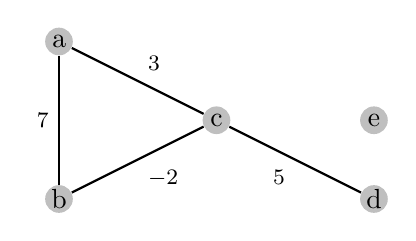
\begin{tikzpicture}[scale=1,auto,swap]
        \node[vertex] (a) at (0,2) {a};
        \node[vertex] (b) at (0,0) {b};
        \node[vertex] (c) at (2,1) {c};
        \node[vertex] (d) at (4,0) {d};
        \node[vertex] (e) at (4,1) {e};
        \draw[edge] (a) -- node[weight] {$7$} (b);
        \draw[edge] (b) -- node[weight] {$-2$} (c);
        \draw[edge] (c) -- node[weight] {$3$} (a);
        \draw[edge] (c) -- node[weight] {$5$} (d);
      \end{tikzpicture}

    \end{columns}
  }
\end{frame}

\begin{frame}
  \frametitle{Quick Review of Graph Terms (2)}

  {\smaller
    \begin{block}{}
      You probably know all of these. If not, ask questions!
    \end{block}

    \begin{columns}[T]
      \column{0.6\textwidth}
      \begin{itemize}
      \item A \structure{path} is a set of vertices connected by edges;
      \item A \structure{cycle} is a path with first and last vertices identical;
      \item \structure{Labelled} graphs and \structure{Isomorphic} graphs;
      \item A \structure{tree} is a acyclical, undirected graph;
      \item A \structure{spanning tree} is a subset of edges from E'
        that form a tree, connecting all nodes $V \in G$;
      \item A \alert{spamming tree} houses very noisy insects in summer;
      \end{itemize}
      \column{0.4\textwidth}
      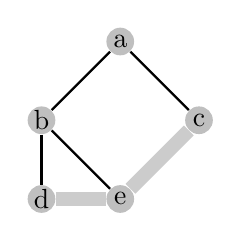
\begin{tikzpicture}[scale=1,auto,swap]
        \node[vertex] (s) at (0,0) {a};
        \node[vertex] (a1) at (-1,-1) {b};
        \node[vertex] (a2) at (1,-1) {c};
        \node[vertex] (b1) at (-1,-2) {d};
        \node[vertex] (b2) at (0,-2) {e};
        \draw[edge] (s) to (a1);
        \draw[edge] (s) to  (a2);
        \draw[edge] (a1) to  (b1);
        \draw[edge] (a1) to  (b2);
        \draw[black edge] (b1) to (b2);
        \draw[black edge] (a2) to (b2);
      \end{tikzpicture}

      \vspace{.5cm}

      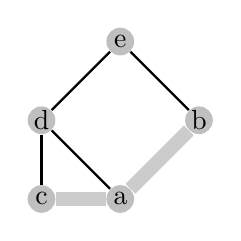
\begin{tikzpicture}[scale=1,auto,swap]
        \node[vertex] (s) at (0,0) {e};
        \node[vertex] (a1) at (-1,-1) {d};
        \node[vertex] (a2) at (1,-1) {b};
        \node[vertex] (b1) at (-1,-2) {c};
        \node[vertex] (b2) at (0,-2) {a};
        \draw[edge] (s) to (a1);
        \draw[edge] (s) to  (a2);
        \draw[edge] (a1) to  (b1);
        \draw[edge] (a1) to  (b2);
        \draw[black edge] (b1) to (b2);
        \draw[black edge] (a2) to (b2);
      \end{tikzpicture}
  \end{columns}}

\end{frame}

\begin{frame}
  \frametitle{Quick Review of Graph Terms (3)}

  {\smaller
    \begin{block}{}
      You probably know all of these. If not, ask questions!
    \end{block}

    \begin{columns}[T]
      \column{0.6\textwidth}
      \begin{itemize}
      \item The \structure{degree} of a node is the number of edges
        connected to it;
      \item Directed graphs have \structure{in-degrees} and
        \structure{out-degrees};
      \item A \structure{bipartite} graph can be divided in two sets
        of unconnected vertices;
      \item A \structure{Match} or \structure{Pairing} is a set of
        edges that connects the nodes in the bipartite graph;
      \end{itemize}
      \column{0.4\textwidth}
      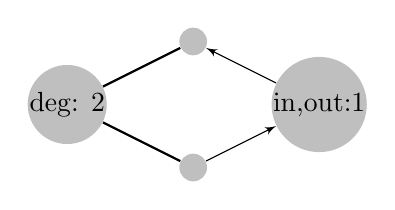
\begin{tikzpicture}[scale=.8,auto,swap]
        \node[vertex] (a) at (0,0) {deg: 2};
        \node[vertex] (b) at (2,1) {};
        \node[vertex] (c) at (2,-1) {};
        \node[vertex] (d) at (4,0) {in,out:1};
        \draw[edge] (a) to (b);
        \draw[edge] (a) to (c);
        \tikzset{edge/.style = {->,>=latex'}}
        \draw[edge] (c) to (d);
        \draw[edge] (d) to (b);
      \end{tikzpicture}
      
      \vspace{.5cm}

      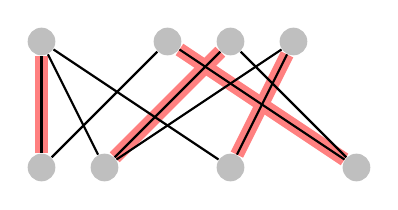
\begin{tikzpicture}[scale=.8,auto,swap]
        \node[vertex] (a1) at (0,0) {};
        \node[vertex] (b1) at (0,2) {};
        \node[vertex] (a2) at (1,0) {};
        \node[vertex] (b2) at (2,2) {};
        \node[vertex] (a3) at (3,0) {};
        \node[vertex] (b3) at (3,2) {};
        \node[vertex] (a4) at (5,0) {};
        \node[vertex] (b4) at (4,2) {};
        \draw[red edge] (a1) to (b1);
        \draw[red edge] (a2) to (b3);
        \draw[red edge] (a3) to (b4);
        \draw[red edge] (a4) to (b2);
        \draw[edge] (a1) to (b1);
        \draw[edge] (a1) to (b2);
        \draw[edge] (a2) to (b1);
        \draw[edge] (a2) to (b3);
        \draw[edge] (a2) to (b4);
        \draw[edge] (a3) to (b1);
        \draw[edge] (a3) to (b4);
        \draw[edge] (a4) to (b3);
        \draw[edge] (a4) to (b2);
      \end{tikzpicture}
  \end{columns}}
\end{frame}

\subsection{graph representation}
\begin{frame}[singleslide,fragile]
  \frametitle{Data Structures for Graphs (1)}
{\smaller
  \begin{block}{Adjacency Matrix - Stores connection between Vertices}
\begin{verbatim}
int adj[100][100];
// adj[i][j] is 0 if no edge between i,j
// adj[i][j] is A if edge of weight A links i,j
\end{verbatim}

    \begin{itemize}
    \item \structure{Pro}: Very simple to program, manipulate;
    \item \alert{Con}: Cannot store multigraph; Wastes space for sparse
      graphs; Requires time $O(V)$ to calculate number of neighbors;
    \end{itemize}
  \end{block}

  \begin{block}{Edge List -- Stores Edges list for each Vertex}
\begin{verbatim}
typedef pair<int,int> ii;
typedef vector<ii> vii;
vector<vii> AdjList;
\end{verbatim}

    \begin{itemize}
    \item \structure{Pro}: $O(V+E)$ space, efficient if graph is sparse; Can store multigraph; 
    \item \alert{Con}: A (bit) more code than Adjacency Matrix
    \end{itemize}
  \end{block}

  }
\end{frame}

\begin{frame}[fragile,singleslide]
  \frametitle{Data Structures for Graphs (2)}
  {\smaller
    \begin{block}{Edge List}
\begin{verbatim}
vector< pair <int,ii>> Edgelist;
\end{verbatim}

    Stores a list of all the edges in the graph. Vertices are implicit
    from the edge list. This is useful for Kruskal's algorithm (which
    we will see later), but otherwise complicates things.
    \end{block}

    \begin{block}{Implicit Graph}
      Some graphs \alert{do not} need to be stored in a special
      structure if they have very clear rules about when two vertices connect.
      \medskip

      Examples:
      \begin{itemize}
      \item A square grid;
      \item Knight's chess moves;
      \item Two vertices $i,j$ connect if $i+j$ is prime;
      \end{itemize}

    \end{block}
  }
\end{frame}


\subsection{Breadth-First-Search/Depth-First-Search}
\begin{frame}
  \frametitle{Searching in a Graph: BFS and DFS}   
  {\small
  Almost all graph problems involve visiting each of its vertices in
  some form. There are two approaches for visiting the nodes in a graph:

  \begin{block}{Depth First Search -- DFS}
    DFS is commonly implemented as a recursive search. For every node
    visited, immediately visit the first edge in it, backtracking when 
    a loop is reached, or no more edges can be followed.
  \end{block}

  \begin{block}{Breadth First Search -- BFS}
    BFS is commonly implemented iterating over a FIFO queue. For every
    node visited, all new edges are put on the back of the queue. Visit
    the next edge at the top of the queue.
  \end{block}}
\end{frame}

\begin{frame}
  \frametitle{BFS/DFS: Visualization}
  \begin{columns}[t]
    \column{0.5\textwidth}
    \begin{exampleblock}{DFS}
      \vspace{0.1cm}
      \begin{center}
      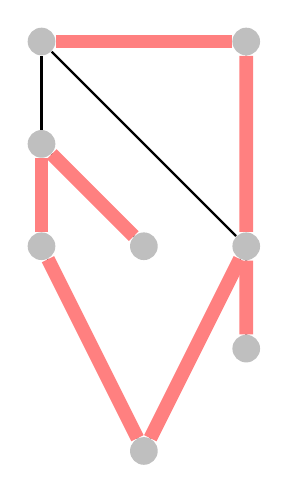
\begin{tikzpicture}[scale=1.3,auto,swap]
        \node[vertex] (a) at (0,0) {};
        \node[vertex] (b) at (2,0) {};
        \node[vertex] (c) at (0,-1) {};
        \node[vertex] (d) at (1,-2) {};
        \node[vertex] (e) at (0,-2) {};
        \node[vertex] (f) at (2,-2) {};
        \node[vertex] (g) at (2,-3) {};
        \node[vertex] (h) at (1,-4) {};
        \draw[edge] (a) to (b);
        \draw[edge] (a) to (c);
        \draw[edge] (a) to (f);
        \draw[edge] (b) to (f);
        \draw[edge] (c) to (d);
        \draw[edge] (c) to (e);
        \draw[edge] (f) to (h);
        \draw[edge] (e) to (h);
        \draw[edge] (f) to (g);
        \draw<2->[red edge] (a) to (b);
        \draw<3->[red edge] (b) to (f);
        \draw<4->[red edge] (f) to (g);
        \draw<5->[red edge] (f) to (h);
        \draw<6->[red edge] (h) to (e);
        \draw<7->[red edge] (e) to (c);
        \draw<8->[red edge] (c) to (d);
      \end{tikzpicture}
      \end{center}
      \vspace{0.1cm}
    \end{exampleblock}
    \column{0.5\textwidth}
    \begin{block}{BFS}
      \vspace{0.1cm}
      \begin{center}
      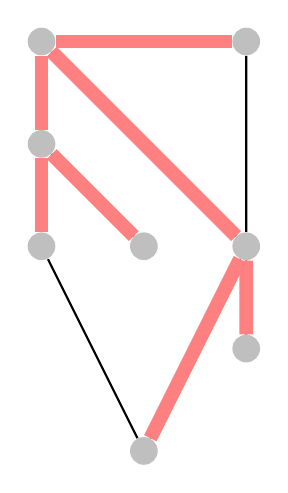
\begin{tikzpicture}[scale=1.3,auto,swap]
        \node[vertex] (a) at (0,0) {};
        \node[vertex] (b) at (2,0) {};
        \node[vertex] (c) at (0,-1) {};
        \node[vertex] (d) at (1,-2) {};
        \node[vertex] (e) at (0,-2) {};
        \node[vertex] (f) at (2,-2) {};
        \node[vertex] (g) at (2,-3) {};
        \node[vertex] (h) at (1,-4) {};
        \draw[edge] (a) to (b);
        \draw[edge] (a) to (c);
        \draw[edge] (a) to (f);
        \draw[edge] (b) to (f);
        \draw[edge] (c) to (d);
        \draw[edge] (c) to (e);
        \draw[edge] (f) to (h);
        \draw[edge] (e) to (h);
        \draw[edge] (f) to (g);
        \draw<2->[red edge] (a) to (b);
        \draw<3->[red edge] (a) to (f);
        \draw<4->[red edge] (a) to (c);
        \draw<5->[red edge] (f) to (g);
        \draw<6->[red edge] (f) to (h);
        \draw<7->[red edge] (c) to (d);
        \draw<8->[red edge] (c) to (e);
      \end{tikzpicture}
      \end{center}
      \vspace{0.1cm}
    \end{block}
  \end{columns}
\end{frame}

\begin{frame}[fragile,singleslide]
  \frametitle{BFS/DFS: Implementation}
  {\smaller
  There are many ways to implement BFS/DFS, here is a suggestion.

  \begin{exampleblock}{DFS}
\begin{verbatim}
vector<int> dfs_vis; // initially all set to UNVISITED
void dfs(int v) {
   dfs_vis = VISITED;
   for (int i; i < (int)Adj_list[v].size(); i++) {
      pair <int,int> u = Adj_list[u][i];
      if (dfs_vis[u.first] == UNVISITED) dfs(v.first)      
}}
\end{verbatim}
  \end{exampleblock}
  \begin{exampleblock}{BFS}
\begin{verbatim}
vector<int> d(V,INF); d[s] = 0; queue<int> q; q.push(s);
while(!q.empty()) {
   u = q.front(); q.pop();
   for (int i=0; i < (int)Adj_list[q].size(); i++) {
   pair <int,int> v = Adj_list[u][i]; //same as dfs
   if (d[v.first] == INF) {   
      d[v.first] = d[u] + 1; q.push(v.first);
}}}
\end{verbatim}
  \end{exampleblock}
  

  }
\end{frame}

\begin{frame}
  \frametitle{Simple BFS/DFS -- UVA 11902: Dominator}
  {\smaller
  \begin{block}{Problem Summary}
    Vertex $X$ \structure{dominates} vertex $Y$ if every path from a
    start vertex $0$ to $Y$ must go through $X$. Determine which
    nodes dominate which other.
  \end{block}}

  \vspace{1cm}

  \begin{center}
    \begin{columns}[T]
      \column{0.5\textwidth}
      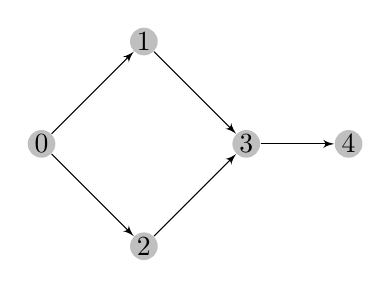
\begin{tikzpicture}[scale=1.3,auto,swap]
        \tikzset{edge/.style = {->,>=latex'}}
        \node[vertex] (a) at (0,0) {0};
        \node[vertex] (b) at (1,1) {1};
        \node[vertex] (c) at (1,-1) {2};
        \node[vertex] (d) at (2,0) {3};
        \node[vertex] (e) at (3,0) {4};
        \draw[edge] (a) to (b);
        \draw[edge] (a) to (c);
        \draw[edge] (b) to (d);
        \draw[edge] (c) to (d);
        \draw[edge] (d) to (e);
      \end{tikzpicture}
      \column{0.5\textwidth}
      \begin{itemize}
      \item 0 dominates all nodes;
      \item 3 dominates 4;
      \item 1 does not dominate 3;

        \bigskip

        How do you solve it?

      \end{itemize}
    \end{columns}
  \end{center}
  %% Simple graph problems (quick modification of DFS/BFS)
  % Dominator: UVA 11902 - Page 148
\end{frame}

\begin{frame}[fragile,singleslide]
  \frametitle{Simple BFS/DFS -- UVA 11902: Dominator}
  
  {\smaller
  \begin{exampleblock}{Solution}
\begin{verbatim}
DFS(0); 
for i in (0:N): 
   if i is reached: dominate[0][i] = 1;

for i in (1:N):
   remove i from graph;
   DFS(0)
   for j in (1:N):
       if (j is not reached) and (dominate[0][j] == 1):
           dominate[i][j] = 1
   return i to graph

\end{verbatim}
  \end{exampleblock}}
  
  \begin{center}
    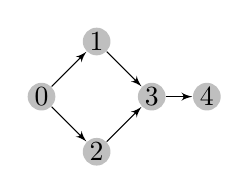
\begin{tikzpicture}[scale=0.7,auto,swap]
      \tikzset{edge/.style = {->,>=latex'}}
      \node[vertex] (a) at (0,0) {0};
      \node[vertex] (b) at (1,1) {1};
      \node[vertex] (c) at (1,-1) {2};
      \node[vertex] (d) at (2,0) {3};
      \node[vertex] (e) at (3,0) {4};
      \draw[edge] (a) to (b);
      \draw[edge] (a) to (c);
      \draw[edge] (b) to (d);
      \draw[edge] (c) to (d);
      \draw[edge] (d) to (e);
    \end{tikzpicture}
  \end{center}
\end{frame}

\section{Common Algorithms}
\subsection{Algorithms using BFS/DFS}
\begin{frame}[fragile,singleslide]
  \frametitle{Common Algorithms: Connected Components}
  {\smaller
    \begin{block}{}
      With small modifications to BFS/DFS, we can solve many simple problems
    \end{block}

    Since a single run of DFS/BFS finds all connected nodes, we can
    use it to find (and count) all the connected components (CC) of an
    \structure{undirected} graph.

    \begin{exampleblock}{}
\begin{verbatim}
numCC = 0;
dfs_num.assign(V,UNVISITED);
for (int = 0; i < V; i++)
   if (dfs_num[i] == UNVISITED)
      cout << "\nCC " << ++numCC << ":"; dfs(i);
      // modify dfs() to print every node it visits
\end{verbatim}
    \end{exampleblock}}

\begin{columns}
  \column{0.5\textwidth}
  \hfill
  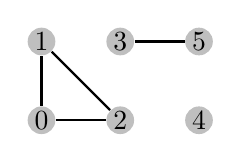
\begin{tikzpicture}[scale=1,auto,swap]
      \node[vertex] (a) at (0,0) {0};
      \node[vertex] (b) at (0,1) {1};
      \node[vertex] (c) at (1,0) {2};
      \node[vertex] (d) at (1,1) {3};
      \node[vertex] (e) at (2,0) {4};
      \node[vertex] (f) at (2,1) {5};
      \draw[edge] (a) to (b);
      \draw[edge] (a) to (c);
      \draw[edge] (b) to (c);
      \draw[edge] (d) to (f);
    \end{tikzpicture}
  \column{0.5\textwidth}
\begin{verbatim}
CC 1: 0 1 2
CC 2: 3 5
CC 3: 4
\end{verbatim}
\end{columns}
\end{frame}

\begin{frame}[fragile,singleslide]
  \frametitle{Flood Fill}
  {\smaller
    \begin{columns}[T]
      \column{0.7\textwidth}
      A simple twear of the BFS (or DFS) can be used to
      \structure{label/color} and count the size of each CC.
      
      \medskip
      
      ``flood fill`` is often used in problems involving implicit 2D
      grids.
      \column{0.3\textwidth}
\begin{verbatim}
####..#
#.###.#
#..@.##
##d.###
#..####
\end{verbatim}
    \end{columns}

  \begin{exampleblock}{}
\begin{verbatim}
int dr[] = {1,1,0,-1,-1,-1,0,1}; // trick to explore an
int dc[] = {0,1,1,1,0,-1,-1,-1}; // implicit NESW graph

int floodfill(int y, int x, char c1, char c2) {
  if (y < 0 || y >= R || x < 0 || x >= C) return 0;
  if (grid[y][x] != c1) return 0;
  int ans = 1;
  grid[y][x] = c2;
  for (int d = 0; d < 8; d++)
     ans += floodfill(y+dr[d], x+dc[d], c1, c2);
  return ans;
}
\end{verbatim}
  \end{exampleblock}
  }
\end{frame}

\begin{frame}[fragile,singleslide]
  \frametitle{Topological Sort (Directed Acyclic Graphs)} 

  {\smaller 
    A Topological sort is a linear ordering of vertices of a DAG so
    that vertex $u$ comes before vertex $v$ if edge $u \rightarrow v$
    exits in the DAG.  Topological Sorts are useful for problems
    involving the ordering of pre-requisites.

    \begin{exampleblock}{Khan's algorithm for Topological sort (modified edge-BFS)}
\begin{verbatim}
Q = queue(); toposort = list();
for j in edge:
   in_degree[j.destination] += 1
for i in node:
   if in_degree[i] == 0: Q.add(i);
while (Q.size() > 0):
   u = Q.dequeue(); toposort.add(u);
   for i in u.out_edges():
       v = i.destination
       in_degree[v] =- 1
       if in_degree[v] == 0:
          Q.add(v);
\end{verbatim}
    \end{exampleblock}

  }
\end{frame}

\begin{frame}[fragile,singleslide]
  \frametitle{Bipartite Check}
  {\smaller
  To check whether a graph is bipartite, we perform a BFS or DFS on the graph, 
  and set the color of every node to black or white, alternatively. Pay 
  attention to collision conditions.

  \begin{exampleblock}{}
\begin{verbatim}
queue<int> q; q.push(s);
vector<int> color(V,INF); color[s] = 0;
bool isBipartite = true;
while (!q.empty() && isBipartite) {
   int u = q.front(); q.pop();
   for (int j=0; j < adj_list[u].size(); j++) {
      pair<int,int> v = adj_list[u][j];
      if (color[v] == INF) {
         color[v.first] = 1 - color[i];
         q.push(v.first);}
      else if (color[v.first] == color[u]) {
         isBipartite = False; 
}}}
\end{verbatim}
  \end{exampleblock}
  }
\end{frame}

\begin{frame}
  \frametitle{Bipartite Check -- Visualization}
  \begin{columns}[t]
    \column{0.5\textwidth}
    \begin{exampleblock}{Testing Bipartite property}
      \vspace{0.1cm}
      \begin{center}
        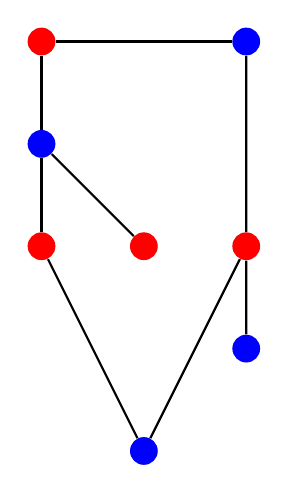
\begin{tikzpicture}[scale=1.3,auto,swap]
          \node[vertex] (a) at (0,0) {};
          \node[vertex] (b) at (2,0) {};
          \node[vertex] (c) at (0,-1) {};
          \node[vertex] (d) at (1,-2) {};
          \node[vertex] (e) at (0,-2) {};
          \node[vertex] (f) at (2,-2) {};
          \node[vertex] (g) at (2,-3) {};
          \node[vertex] (h) at (1,-4) {};
          \draw[edge] (a) to (b);
          \draw[edge] (a) to (c);
          \draw[edge] (b) to (f);
          \draw[edge] (c) to (d);
          \draw[edge] (c) to (e);
          \draw[edge] (f) to (h);
          \draw[edge] (e) to (h);
          \draw[edge] (f) to (g);
          \uncover<2->{\node[red vertex] (a1) at (0,0) {};}
          \uncover<3->{\node[blue vertex] (b1) at (2,0) {};}
          \uncover<3->{\node[blue vertex] (c1) at (0,-1) {};}
          \uncover<4->{\node[red vertex] (d1) at (1,-2) {};}
          \uncover<4->{\node[red vertex] (e1) at (0,-2) {};}
          \uncover<4->{\node[red vertex] (f1) at (2,-2) {};}
          \uncover<5->{\node[blue vertex] (g1) at (2,-3) {};}
          \uncover<5->{\node[blue vertex] (h1) at (1,-4) {};}
        \end{tikzpicture}
      \end{center}
      \vspace{0.1cm}
    \end{exampleblock}
    \column{0.5\textwidth}
    \uncover<6->{
    \begin{exampleblock}{Rearranging the nodes}
      \vspace{0.1cm}
      \begin{center}
        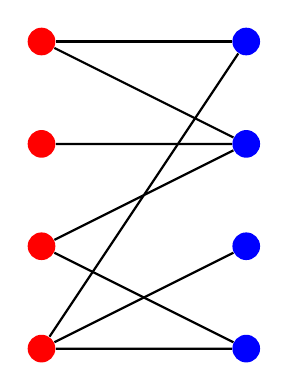
\begin{tikzpicture}[scale=1.3,auto,swap]
          \node[red vertex] (a) at (0,0) {};
          \node[blue vertex] (b) at (2,0) {};
          \node[blue vertex] (c) at (2,-1) {};
          \node[red vertex] (d) at (0,-1) {};
          \node[red vertex] (e) at (0,-2) {};
          \node[red vertex] (f) at (0,-3) {};
          \node[blue vertex] (g) at (2,-2) {};
          \node[blue vertex] (h) at (2,-3) {};
          \draw[edge] (a) to (b);
          \draw[edge] (a) to (c);
          \draw[edge] (b) to (f);
          \draw[edge] (c) to (d);
          \draw[edge] (c) to (e);
          \draw[edge] (f) to (h);
          \draw[edge] (e) to (h);
          \draw[edge] (f) to (g);
        \end{tikzpicture}
      \end{center}
      \vspace{0.1cm}
    \end{exampleblock}}
  \end{columns}
\end{frame}

\begin{frame}
  \frametitle{Articulation Points and Bridges}
  {\smaller
    \begin{block}{Problem Description}
      In an undirected graph G:
      \begin{itemize}
      \item A verted V is an \structure{Articulation Point} if removing V would make G disconnected.
      \item An edge E is a \structure{Bridge} if removing E would make G disconnected.
      \end{itemize}
    \end{block}
    \begin{center}
        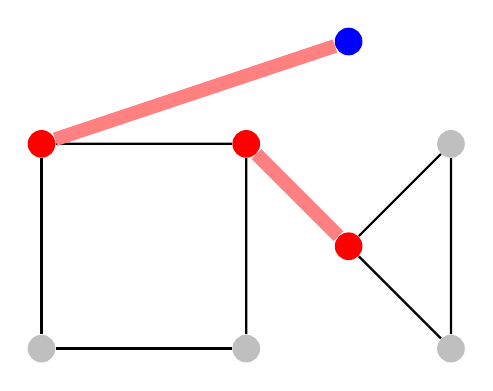
\begin{tikzpicture}[scale=1.3,auto,swap]
          \node[vertex] (a) at (0,0) {};
          \node[vertex] (b) at (2,0) {};
          \node[red vertex] (c) at (0,2) {};
          \node[red vertex] (d) at (2,2) {};
          \node[red vertex] (e) at (3,1) {};
          \node[vertex] (f) at (4,0) {};
          \node[vertex] (g) at (4,2) {};
          \node[blue vertex] (h) at (3,3) {};
          \draw[edge] (a) to (b);
          \draw[edge] (a) to (c);
          \draw[edge] (c) to (d);
          \draw[edge] (d) to (b);
          \draw[red edge] (d) to (e);
          \draw[edge] (e) to (f);
          \draw[edge] (f) to (g);
          \draw[edge] (g) to (e);
          \draw[red edge] (c) to (h);
        \end{tikzpicture}
      \end{center}
  }
\end{frame}

\begin{frame}
  \frametitle{Articulation Points and Bridges: Algorithm}
  {\smaller
    \begin{block}{Complete Search algorithm for Articulation Points}
      \begin{enumerate}
      \item Run DFS/BFS, and count the number of CC in the graph;
      \item For each vertex $v$, remove $v$ and run DFS/BFS again;
      \item If the number of CC increases, $v$ is a connection point;
      \end{enumerate}
      Since DFS/BFS is $O(V+E)$, this algorithm runs in $O(V^2+EV)$.
    \end{block}
    
    \bigskip

    \hfill ... but we can do better!
  }
\end{frame}

% TODO: Make my own image for the DFS articulation detection algorithm
\begin{frame}
  \frametitle{Tarjan's DFS variant for Articulation point (O(V+E))}
  {\smaller
    \begin{exampleblock}{Tarjan Variant: $O(V+E)$}
      Main idea: Add extra data to the DFS to detect articulations.
    \end{exampleblock}
      \begin{center}
        \includegraphics[width=0.9\textwidth]{../img/graph_articulation}
      \end{center}
    \begin{itemize}
    \item \structure{dfs\_num[]}: Recieves the number of the iteration
      when this node was reached for the first time;
    \item \structure{dfs\_low[]}: Recieves the lowest dfs\_num[] which
      can be reached if we start the DFS from here;
    \item For any neighbors $u,v$, if dfs\_low[$v$] >= dfs\_num[$u$],
      then $u$ is an articulation node.
    \end{itemize}
  }
\end{frame}

\begin{frame}[fragile,singleslide]
  \frametitle{Tarjan's DFS variant for Articulation point (2)}
  \begin{center}
    \includegraphics[width=0.6\textwidth]{../img/graph_articulation}
  \end{center}
  
{\tiny
  \begin{exampleblock}{}
\begin{verbatim}
void dfs_a(u){
   dfs_num[u] = dfs_low[u] = IterationCounter++;   // dfs_num[u] is a simple counter
   for (int i = 0; i < AdjList[u].size(); i++){
      v = AdjList[u][i];
      if (dfs_num[v] == UNVISITED) {
         dfs_parent[v] = u;                        // store parent
         if (u == 0) rootChildren++:               // special case for root node

         dfs_a(v);
         if (dfs_low[a] >= dfs_num[u])
            articulation_vertex[u] = true;
         dfs_low[u] = min(dfs_low[u],dfs_low[v])

      else if (v != dfs_parent[u])                 // found a cycle edge
         dfs_low[u] = min(dfs_low[u],dfs_num[v])
}}
\end{verbatim}
  \end{exampleblock}}
\end{frame}

\begin{frame}
  \frametitle{Strongly Connected Components (Directed Graph)}
  {\smaller
    \begin{block}{Problem Description}
      On a directed graph $G$, a Strongly Connected Component (SCC) is
      a subset $G'$ where for every pair of nodes $a,b \in G'$, there is both 
      a path $a \rightarrow b$ and a path $b \rightarrow a$.
    \end{block}


\begin{columns}[t]
    \column{0.5\textwidth}
    \begin{exampleblock}{One CC}
      \vspace{0.1cm}
      \begin{center}
        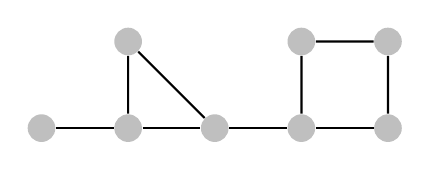
\begin{tikzpicture}[scale=1.1,auto,swap]
          \node[vertex] (a) at (0,0) {};
          \node[vertex] (b) at (1,0) {};
          \node[vertex] (c) at (2,0) {};
          \node[vertex] (d) at (1,1) {};
          \node[vertex] (e) at (3,0) {};
          \node[vertex] (f) at (4,0) {};
          \node[vertex] (g) at (4,1) {};
          \node[vertex] (h) at (3,1) {};
          \draw[edge] (a) to (b);
          \draw[edge] (b) to (c);
          \draw[edge] (c) to (d);
          \draw[edge] (d) to (b);
          \draw[edge] (c) to (e);
          \draw[edge] (e) to (f);
          \draw[edge] (f) to (g);
          \draw[edge] (g) to (h);
          \draw[edge] (h) to (e);
        \end{tikzpicture}
      \end{center}
      \vspace{0.1cm}
    \end{exampleblock}
    \column{0.5\textwidth}
    \begin{exampleblock}{Three SCC}
      \vspace{0.1cm}
      \begin{center}
        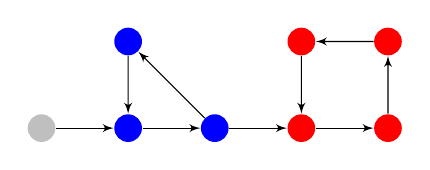
\begin{tikzpicture}[scale=1.1,auto,swap]
          \tikzset{edge/.style = {->,>=latex'}}
          \node[vertex] (a) at (0,0) {};
          \node[blue vertex] (b) at (1,0) {};
          \node[blue vertex] (c) at (2,0) {};
          \node[blue vertex] (d) at (1,1) {};
          \node[red vertex] (e) at (3,0) {};
          \node[red vertex] (f) at (4,0) {};
          \node[red vertex] (g) at (4,1) {};
          \node[red vertex] (h) at (3,1) {};
          \draw[edge] (a) to (b);
          \draw[edge] (b) to (c);
          \draw[edge] (c) to (d);
          \draw[edge] (d) to (b);
          \draw[edge] (c) to (e);
          \draw[edge] (e) to (f);
          \draw[edge] (f) to (g);
          \draw[edge] (g) to (h);
          \draw[edge] (h) to (e);
        \end{tikzpicture}
      \end{center}
      \vspace{0.1cm}
    \end{exampleblock}
  \end{columns}
  }
\end{frame}

\begin{frame}
  \frametitle{Strongly Connected Components -- Algorithm} 

  We can use a simple modification of the algorithm for bridges and
  articulation points:

  \begin{itemize}
    \item Every time we visit a new node, put that node in a stack $S$;
    \item When we finish visiting a node $i$, test if dfs\_num[$i$] == dfs\_min[$i$].
    \item If the above condition is true, $i$ is the root of the
      SCC. Pop all vertices in the stack as part of the SCC.
  \end{itemize}
\end{frame}

%%%%%%%%%%%%%%%%%%%%%%%%%%%%%%%%%%%%%%%%%%%%%%%

\section{Spanning Tree}
\subsection{Introduction}
\begin{frame}
  \frametitle{Minimum Spanning Trees (MST)}

  {\smaller
  \begin{block}{Definition}
    A \structure{Spanning Tree} is a subset $E'$ from graph $G$ so
    that all vertices are connected without cycles.

    \medskip

    A \structure{Minimum Spanning Tree} is a spanning tree where the
    sum of edge's weights is minimal.    
  \end{block}
  }

  \begin{columns}[T]
    \column{0.3\textwidth}
    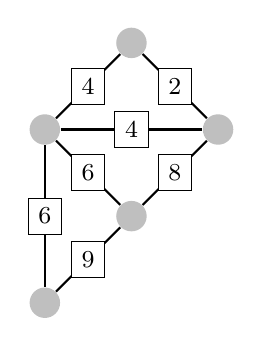
\begin{tikzpicture}[transform shape,label/.style={thin, draw=black, align=center,fill=white,font=\smaller},scale=1.1]
      \node[vertex] (a) at (0,0) {};
      \node[vertex] (b) at (1,1) {};
      \node[vertex] (c) at (2,0) {};
      \node[vertex] (d) at (1,-1) {};
      \node[vertex] (e) at (0,-2) {};
      \draw[edge] (a) -- node[label] {$4$} (b);
      \draw[edge] (b) -- node[label] {$2$} (c);
      \draw[edge] (a) -- node[label] {$4$} (c);
      \draw[edge] (a) -- node[label] {$6$} (d);
      \draw[edge] (c) -- node[label] {$8$} (d);
      \draw[edge] (a) -- node[label] {$6$} (e);
      \draw[edge] (d) -- node[label] {$9$} (e);
    \end{tikzpicture}
    \column{0.3\textwidth}
    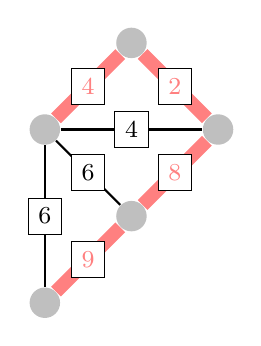
\begin{tikzpicture}[transform shape,label/.style={thin, draw=black, align=center,fill=white,font=\smaller},scale=1.1]
      \node[vertex] (a) at (0,0) {};
      \node[vertex] (b) at (1,1) {};
      \node[vertex] (c) at (2,0) {};
      \node[vertex] (d) at (1,-1) {};
      \node[vertex] (e) at (0,-2) {};
      \draw[red edge] (a) -- node[label] {$4$} (b);
      \draw[red edge] (b) -- node[label] {$2$} (c);
      \draw[edge] (a) -- node[label] {$4$} (c);
      \draw[edge] (a) -- node[label] {$6$} (d);
      \draw[red edge] (c) -- node[label] {$8$} (d);
      \draw[edge] (a) -- node[label] {$6$} (e);
      \draw[red edge] (d) -- node[label] {$9$} (e);
    \end{tikzpicture}
    \column{0.3\textwidth}
    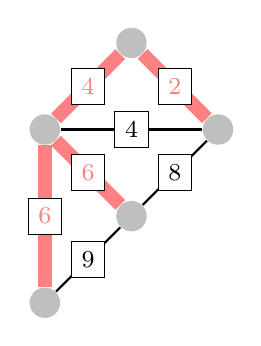
\begin{tikzpicture}[transform shape,label/.style={thin, draw=black, align=center,fill=white,font=\smaller},scale=1.1]
      \node[vertex] (a) at (0,0) {};
      \node[vertex] (b) at (1,1) {};
      \node[vertex] (c) at (2,0) {};
      \node[vertex] (d) at (1,-1) {};
      \node[vertex] (e) at (0,-2) {};
      \draw[red edge] (a) -- node[label] {$4$} (b);
      \draw[red edge] (b) -- node[label] {$2$} (c);
      \draw[edge] (a) -- node[label] {$4$} (c);
      \draw[red edge] (a) -- node[label] {$6$} (d);
      \draw[edge] (c) -- node[label] {$8$} (d);
      \draw[red edge] (a) -- node[label] {$6$} (e);
      \draw[edge] (d) -- node[label] {$9$} (e);
    \end{tikzpicture}
  \end{columns}
\end{frame}

\begin{frame}
  \frametitle{MST -- Use cases and Algorithms}
  {\small
  \begin{block}{Problems using MST}
    Problems using MST usually involve calculating the minimum costs
    of infrastructure such as roads or networks. 
    
    \medskip

    Some variations may require you to find the \alert{maximum}
    spanning tree, or define some edges that \alert{must} be taken in advance.
  \end{block}

  \begin{exampleblock}{Algorithms for MST}
    The two main algorithms for calculating the MST are the
    \structure{Kruskal}'s algorithms and the \structure{Prim}'s
    algorithms.

    \medskip

    Both are greedy algorithms that add edges to the MST in weight order.
  \end{exampleblock}
    }
\end{frame}

\begin{frame}
  \frametitle{Kruskal's Algorithm}
  \begin{block}{Outline}
    Kruskal's algorithms sorts all edges by their weight, and try to
    add each edge to the MST, checking whether adding that edge would
    create a cycle.
  \end{block}

  \begin{columns}[T]
    \column{0.5\textwidth}
    \begin{enumerate}
    \item Sort all edges;
    \item If smallest edge does not create a cycle, add to MST;
    \item If smallest edge creates a cycle, remove it from list;
    \item Go to 2;
    \end{enumerate}
    \column{0.5\textwidth}
    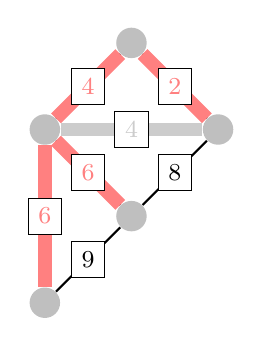
\begin{tikzpicture}[transform shape,label/.style={thin, draw=black, align=center,fill=white,font=\smaller},scale=1.1]
      \node[vertex] (a) at (0,0) {};
      \node[vertex] (b) at (1,1) {};
      \node[vertex] (c) at (2,0) {};
      \node[vertex] (d) at (1,-1) {};
      \node[vertex] (e) at (0,-2) {};
      \draw[edge] (a) -- node[label] {$4$} (b);
      \draw[edge] (b) -- node[label] {$2$} (c);
      \draw[edge] (a) -- node[label] {$4$} (c);
      \draw[edge] (a) -- node[label] {$6$} (d);
      \draw[edge] (c) -- node[label] {$8$} (d);
      \draw[edge] (a) -- node[label] {$6$} (e);
      \draw[edge] (d) -- node[label] {$9$} (e);
      \draw<2->[red edge] (b) -- node[label] {$2$} (c);
      \draw<3->[red edge] (a) -- node[label] {$4$} (b);
      \draw<4->[black edge] (a) -- node[label] {$4$} (c);
      \draw<4->[red edge] (a) -- node[label] {$6$} (d);
      \draw<5->[red edge] (a) -- node[label] {$6$} (e);
    \end{tikzpicture}
  \end{columns}
\end{frame}

\begin{frame}[fragile,singleslide]
  \frametitle{Kruskal's Algorithm -- Implementation}
{\smaller
\begin{exampleblock}{}
\begin{verbatim}
vector<pair<int, pair<int,int>> Edgelist; 
sort(Edgelist.begin(),Edgelist.end());
int mst_cost = 0; 
UnionFind UF(V);
  // note 1: Pair object has built-in comparison;
  // note 2: Need to implement UnionSet class;

for (int i = 0; i < Edgelist.size(); i++) {
   pair <int, pair <int,int>> front = Edgelist[i];
   if (!UF.isSameSet(front.second.first,
                     front.second.second)) {
      mst_cost += front.first;
      UF.unionSet(front.second.first,front.second.second)
   }}

cout << "MST Cost: " << mst_cost << "\n"
\end{verbatim}
\end{exampleblock}
}
\end{frame}

\begin{frame}
  \frametitle{Prim's Algorithm}
  {\small
  \begin{block}{Outline}
    Prim's algorith adds nodes to the MST one at a time, and keeps the
    edges connected to those nodes in a \structure{priority queue}. It
    then tests each edge in the priority queue to add more nodes to
    the MST, avoiding cycles.
  \end{block}

  \begin{columns}[T]
    \column{0.5\textwidth}
    \begin{enumerate}
    \item Add node 0 to MST;
    \item Add all edges from new node to Priority Queue;
    \item Visit smallest edge in Queue;
    \item If the edge leades to a new node, add it to MST;
    \item Add new edges to Queue;
    \item Go to 3;
    \end{enumerate}
    \column{0.5\textwidth}
    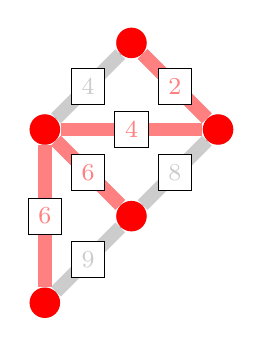
\begin{tikzpicture}[transform shape,label/.style={thin, draw=black, align=center,fill=white,font=\smaller},scale=1.1]
      \node[vertex] (a) at (0,0) {};
      \node[vertex] (b) at (1,1) {};
      \node[vertex] (c) at (2,0) {};
      \node[vertex] (d) at (1,-1) {};
      \node[vertex] (e) at (0,-2) {};
      \draw[edge] (a) -- node[label] {$4$} (b);
      \draw[edge] (b) -- node[label] {$2$} (c);
      \draw[edge] (a) -- node[label] {$4$} (c);
      \draw[edge] (a) -- node[label] {$6$} (d);
      \draw[edge] (c) -- node[label] {$8$} (d);
      \draw[edge] (a) -- node[label] {$6$} (e);
      \draw[edge] (d) -- node[label] {$9$} (e);
      \uncover<2->{
      \node[red vertex] (a1) at (0,0) {};
      \draw[black edge] (a) -- node[label] {$4$} (b);
      \draw[black edge] (a) -- node[label] {$4$} (c);
      \draw[black edge] (a) -- node[label] {$6$} (d);
      \draw[black edge] (a) -- node[label] {$6$} (e);
      }

      \uncover<3->{
        \node[red vertex] (c1) at (2,0) {};
        \draw[red edge] (a) -- node[label] {$4$} (c);
        \draw[black edge] (c) -- node[label] {$8$} (d);
        \draw[black edge] (b) -- node[label] {$2$} (c);
      }
      \uncover<4->{
        \node[red vertex] (b1) at (1,1) {};
        \draw[red edge] (b) -- node[label] {$2$} (c);
      }

      \uncover<5->{
        \node[red vertex] (d1) at (1,-1) {};
        \draw[red edge] (a) -- node[label] {$6$} (d);
        \draw[black edge] (d) -- node[label] {$9$} (e);
      }
      
      \uncover<6->{
        \node[red vertex] (e1) at (0,-2) {};
        \draw[red edge] (a) -- node[label] {$6$} (e);
      }
    \end{tikzpicture}
  \end{columns}
  }
\end{frame}

\begin{frame}[fragile,singleslide]
  \frametitle{Prim's Algorithm -- Implementation}
{\smaller
\begin{exampleblock}{}
\begin{verbatim}
vector <int> taken;
priority_queue <pair <int,int>> pq;

void process (int v) {
   taken[v] = 1;
   for (int j = 0; j < (int)AdjList[v].size(); j++) {
      pair <int,int> ve = AdjList[v][j];
      if (!taken[ve.first]) 
         pq.push(pair <int,int> (-ve.second,-ve.second)
}}
taken.assign(V,0);
process(0);
mst_cost = 0;

while (!pq.empty()) {
  vector <int,int> pq.top(); pq.pop();
  u = -front.secont, w = -front.first;
  if (!taken[u]) mst_cost += w, process(u);
}
\end{verbatim}
\end{exampleblock}
}
\end{frame}

\subsection{Other MST Problems}

\begin{frame}
  \frametitle{MST variant 1 -- Maximum Spanning tree}

  {\smaller
    \begin{block}{}
      The \structure{Maximum Spanning Tree} variant requires the spanning
      tree to have maximum possible weight.
      
      \bigskip
      
      It is very easy to implement the Maximum MST by reversing the sort
      order of the edges (Kruskal), or the weighting of the priority Queue
      (Prim).
    \end{block}

  \medskip

  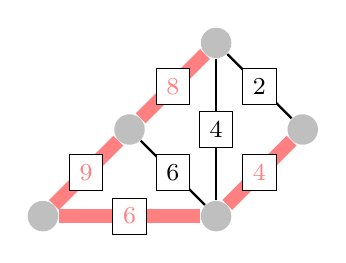
\begin{tikzpicture}[transform shape,label/.style={thin, draw=black, align=center,fill=white,font=\smaller},scale=1.1]
      \node[vertex] (a) at (0,0) {};
      \node[vertex] (b) at (1,1) {};
      \node[vertex] (c) at (0,2) {};
      \node[vertex] (d) at (-1,1) {};
      \node[vertex] (e) at (-2,0) {};
      \draw[red edge] (a) -- node[label] {$4$} (b);
      \draw[edge] (b) -- node[label] {$2$} (c);
      \draw[edge] (a) -- node[label] {$4$} (c);
      \draw[edge] (a) -- node[label] {$6$} (d);
      \draw[red edge] (c) -- node[label] {$8$} (d);
      \draw[red edge] (a) -- node[label] {$6$} (e);
      \draw[red edge] (d) -- node[label] {$9$} (e);
  \end{tikzpicture}}
\end{frame}

\begin{frame}
  \frametitle{MST variant 2 -- Minimum Spanning Subgraph, Forest}
  {\smaller
    \begin{block}{}
      In one importante variant of the MST, a subset of edges or
      vertices are pre-selected.

      \begin{itemize}
      \item In the case of pre-selected vertices, add them to the
        ``taken'' list in Kruskal's algorithm before starting;
      \item In the case of edges, add the end vertices to the
        ``taken'' list;
      \item What if you are given a \alert{number of Connected Components}?
      \end{itemize}
    \end{block}
    \begin{center}
      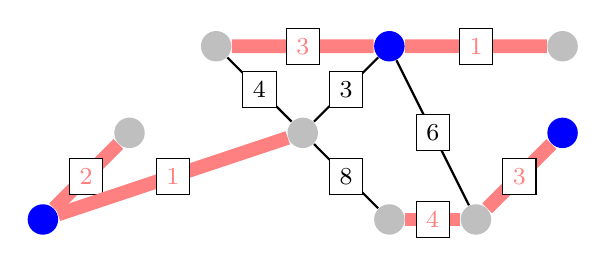
\begin{tikzpicture}[transform shape,label/.style={thin, draw=black, align=center,fill=white,font=\smaller},scale=1.1]
        \node[blue vertex] (a) at (0,0) {};
        \node[vertex] (b) at (1,1) {};
        \node[vertex] (c) at (2,2) {};
        \node[vertex] (d) at (3,1) {};
        \node[vertex] (e) at (4,0) {};
        \node[blue vertex] (f) at (4,2) {};
        \node[vertex] (g) at (5,0) {};
        \node[vertex] (h) at (6,2) {};
        \node[blue vertex] (i) at (6,1) {};
        \draw[red edge] (a) -- node[label] {$2$} (b);
        \draw[red edge] (a) -- node[label] {$1$} (d);
        \draw[edge] (d) -- node[label] {$4$} (c);
        \draw[edge] (d) -- node[label] {$8$} (e);
        \draw[edge] (d) -- node[label] {$3$} (f);
        \draw[red edge] (c) -- node[label] {$3$} (f);
        \draw[edge] (f) -- node[label] {$6$} (g);
        \draw[red edge] (e) -- node[label] {$4$} (g);
        \draw[red edge] (f) -- node[label] {$1$} (h);
        \draw[red edge] (g) -- node[label] {$3$} (i);
      \end{tikzpicture}
    \end{center}
  }
\end{frame}

\begin{frame}
  \frametitle{MST Variant 3 -- $n$th Best MST}
  {\smaller
  \begin{block}{Problem Definition}
    Consider that you can order MST by their costs: $G_1, G_2, \ldots,
    G_n$.  This variant asks you to calculate the $n^{th}$ best
    spanning tree.    
  \end{block}

  \bigskip

  Basic Idea:
  \begin{itemize}
    \item Calculate the MST (using Kruskal or Prim);
    \item For every edge in the MST, remove that edge from the graph
      and calculate a new MST;
    \item The new MST with minimum weight is the $2^{nd}$ best MST;
  \end{itemize}
}
\end{frame}

\begin{frame}
  \frametitle{MST Variant 4 -- Min-max (or Max-min)}

  {\smaller

  \begin{center}
      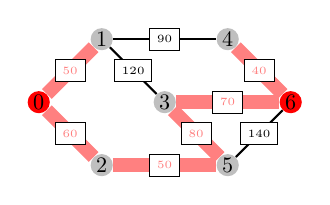
\begin{tikzpicture}[transform shape,label/.style={thin, draw=black, align=center,fill=white,font=\tiny},scale=0.8]
        \node[red vertex] (a) at (0,0) {0};
        \node[vertex] (b) at (1,1) {1};
        \node[vertex] (c) at (1,-1) {2};
        \node[vertex] (d) at (2,0) {3};
        \node[vertex] (e) at (3,1) {4};
        \node[vertex] (f) at (3,-1) {5};
        \node[red vertex] (g) at (4,0) {6};
        \draw[red edge] (a) -- node[label] {$50$} (b);
        \draw[red edge] (a) -- node[label] {$60$} (c);
        \draw[edge] (b) -- node[label] {$120$} (d);
        \draw[edge] (b) -- node[label] {$90$} (e);
        \draw[red edge] (c) -- node[label] {$50$} (f);
        \draw[red edge] (d) -- node[label] {$80$} (f);
        \draw[red edge] (d) -- node[label] {$70$} (g);
        \draw[red edge] (e) -- node[label] {$40$} (g);
        \draw[edge] (f) -- node[label] {$140$} (g);
      \end{tikzpicture}
    \end{center}
  
  \begin{block}{Problem Definition}
    Given two vertices $i,j$, find a path $i \rightarrow j$ so that
    the cost of the most expensive edge is minimized;

    \medskip

    Another way to write this problem is: Find the cheapest path where
    the cost of the path is the cost of the most expensive edge.
  \end{block}

  \begin{exampleblock}{How to solve}
    The MST finds the path that connects all nodes while keeping the
    cost of individual edges minimal. 

    \medskip
    
    To solve the minimax problem, we calculate the MST for $G$, and
    then find the path from $i$ to $j$ in the MST.
  \end{exampleblock}
  }
\end{frame}


\section{Conclusion}
\subsection{Conclusion}
\begin{frame}
  \frametitle{Summary}
  \begin{itemize}
  \item Graphs come in a wide variety of types;
  \item Graph problems also have many different types;
  \item Most problems involve small modifications of DFS and BFS;
  \end{itemize}
\end{frame}

\begin{frame}
  \frametitle{This Week's Problems}
  \begin{itemize}
  \item Dominator;
  \item Knight in a War grid;
  \item Wetlands in Florida;
  \item Battleships;
  \item Pick up Sticks;
  \item Place the Guards;
  \item Street Directions;
  \item Dominos;
  \item Freckles;
  \item Artic Network;
  \end{itemize}
\end{frame}

\begin{frame}
  \frametitle{Problem Hints (0)}
  \begin{itemize}
  \item All the problems this week (and next week!) include graphs,
    and probably need BFS and/or DFS;

    \medskip

  \item Prepare a ``template'' of an Adjacency list and DFS/BFS, and
    put it in the code before starting;

    \medskip

  \item Try to draw the problem on paper before coding;

    \medskip

  \item Remember to test ``tricky'' cases: Graphs with 1 node,
    disconnected graphs, self-edges, multi-edges;
  \end{itemize}
\end{frame}

\begin{frame}
  \frametitle{Problem Hints (1)}
  {\smaller
  \begin{block}{Dominator}
    \begin{itemize}
    \item Remember: A node is not dominated by anyone if it is not connected to the root (node 0);
    \item Basic algorithm discussed in class: Calculate all nodes
      reachable from root. Then remove one node at a time, and node which ones are not reachable anymore;
    \item If removing node $i$ makes node $j$ not reachable, then $i$ dominates $j$.
    \item To ``remove'' a node, modify the DFS(root,i) so that it returns if $i$ is reached;
    \end{itemize}
  \end{block}
  }
\end{frame}

\begin{frame}
  \frametitle{Problem Hints (2)}
  {\smaller
  \begin{block}{Knight in a War Grid}
    \begin{itemize}
    \item The problem only wants to know which squares are reachable,
      it is not worried about minimum distance;
    \item Be careful, $M$ or $N$ can be zero!
    \item Be careful, if $M == N$, the graph becomes multigraph!
    \item This graph is implicit, the connections are given by the
      knight step, the board size, and the impossible squares;
    \end{itemize}
  \end{block}
  }
\end{frame}

\begin{frame}
  \frametitle{Problem Hints (3)}
  {\smaller
  \begin{block}{Wetlands of Florida}
    \begin{itemize}
      \item Make a graph with 0 and 1 indicating water or no water;
      \item Flood-fill the graph at the requested location;
      \item Multiple-case input is a bit hard to read, make sure to test that;
    \end{itemize}
  \end{block}
  \begin{block}{Battleships}
    \begin{itemize}
      \item Scan the graph (double fors). 
      \item For each unvisited 'x' or '@', flood fill the ship (mark
        visited) and add the ship;
      \item A ship with only @'s should not be counted.
    \end{itemize}
  \end{block}}
\end{frame}

\begin{frame}
  \frametitle{Problem Hints (4)}
  {\smaller
  \begin{block}{Pick up sticks}
    \begin{itemize}
    \item The input gives you directed nodes. 
    \item Try to build a topological order (follow the class code)
    \item Any order is fine. If you find a cycle, print ``impossible''
    \end{itemize}
  \end{block}
  \begin{block}{Palace Guards}
    \begin{itemize}
    \item Each junction is a node, each street is an edge. 
    \item We have junctions with guards and without guards. (No guard can be near each other)
    \item There is a solution if the graph is bipartite!
    \item How do you calculate the smallest number of guards?
    \end{itemize}
  \end{block}}
\end{frame}

\begin{frame}
  \frametitle{Problem Hints (5)}
  {\smaller
  \begin{block}{Street Directions}
    \begin{itemize}
    \item We have to convert two way streets to one way streets 
    \item Undirected graph to directd graph. 
    \item When is a 2-way street \alert{necessary}?
    \item How can you generate 1 way streets?
    \item Hint: you need to draw the graph on paper
    \end{itemize}
  \end{block}
  \begin{block}{Dominos}
    \begin{itemize}
    \item The dominos falling is a directed graph. 
    \item Each domino that falls, we visit one node.
    \item How many nodes do we need to start, to visit all nodes?
    \end{itemize}
  \end{block}}
\end{frame}

\begin{frame}
  \frametitle{Problem Hints (6)}
  \begin{block}{Freckles}
    \begin{itemize}
    \item The problem requires the minimum ink (cost) among all freckles;
    \item This is straight up MST code;
    \item Be careful when rounding up values;
    \end{itemize}    
  \end{block}
  \begin{block}{Arctic Network}
    \begin{itemize}
    \item Also wants to calculate the MST (minimum radio power necessary);
    \item However, we can use $S$ ``satellite'' links, which cost 0;
    \item Remember that two stations need a satellite link to talk;
    \end{itemize}
  \end{block}
\end{frame}


\begin{frame}
  \frametitle{Next Week}
  More Graphs!
  \begin{itemize}
  \item Shortest Paths (Single Source and All Pairs);
  \item Network Flow (and related problems);
  \item Graph Matching (bipartite matching, etc) (and related problems);
  \end{itemize}
\end{frame}

\begin{frame}[fragile,singleslide]
  \frametitle{EXTRA: Union Find Disjoint Set}
  
  {\tiny
    \begin{exampleblock}{Union Find Class}
\begin{verbatim}
class UnionFind {
private: vector<int> p, rank;
public: 
   UnionFind(int N) {
      rank.assign(N,0);
      p.assign(N,0); for (int i=0; i<N; i++) p[i]=i;}
   int findSet(int i) {
      return (p[i] == i? i : (pi[i] = findSet(p[i]))); }
   bool isSameSet(int i, int j) { 
      return findSet(i) == findSet (j); }
   void unionSet(int i, int j) {
      is (!isSameSet(int i, int j) { 
         int x = findSet(i), y = findSet(j);
         if (rank[x] > rank[y]) 
            p[y] = x;
         else { 
            p[x] = y;
            if (rank[x] == rank[y]) rank[y]++; }
   }}
};
\end{verbatim}
    \end{exampleblock}
  }
\end{frame}

%% TODO: Extra: Why study graph problems
% Human Networks (Scale-free Networks)
% State Machines (Computation models, theory)
% Dependence Graphs (Compilers, Pipelining, Scheduling)
% Grammar Graphs (Compilers, NLP)
\end{document}

